\XtoCBlock{Real2Int}
\label{block:Real2Int}
\begin{figure}[H]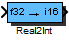
\includegraphics{Real2Int}\end{figure} 

\begin{XtoCtabular}{Inports}
In & Real input\tabularnewline
\hline
\end{XtoCtabular}


\begin{XtoCtabular}{Outports}
Out & Integer output\tabularnewline
\hline
\end{XtoCtabular}

\begin{XtoCtabular}{Mask Parameters}
Scale & Scaling factor from real to integer\tabularnewline
\hline
\end{XtoCtabular}

\subsubsection*{Description:}
Conversion block from real (floating point) datatypes to integer (fixed point) datatypes.

  Out = In / Scale 

% include optional documentation file
\InputIfFileExists{\XcHomePath/Library/General/Doc/Real2Int_Info.tex}{\vspace{1ex}}{}

\subsubsection*{Implementations:}
\begin{tabular}{l l}
\textbf{Float32\_FiP8} & 32 Floating Point to 8 Bit Fixed Point Implementation\tabularnewline
\textbf{Float32\_FiP16} & 32 Floating Point to 16 Bit Fixed Point Implementation\tabularnewline
\textbf{Float32\_FiP32} & 32 Floating Point to 32 Bit Fixed Point Implementation\tabularnewline
\textbf{Float64\_FiP8} & 64 Floating Point to 8 Bit Fixed Point Implementation\tabularnewline
\textbf{Float64\_FiP16} & 64 Floating Point to 16 Bit Fixed Point Implementation\tabularnewline
\textbf{Float64\_FiP32} & 64 Floating Point to 32 Bit Fixed Point Implementation\tabularnewline
\end{tabular}

\XtoCImplementation{Float32\_FiP8}
\index{Block ID!208}
\nopagebreak[0]
% Implementation details
\begin{tabular}{l l}
\textbf{Name} & Float32\_FiP8 \tabularnewline
\textbf{ID} & 208 \tabularnewline
\textbf{Revision} & 0.1 \tabularnewline
\textbf{C filename} & Real2Int\_Float32\_FiP8.c \tabularnewline
\textbf{H filename} & Real2Int\_Float32\_FiP8.h \tabularnewline
\end{tabular}
\vspace{1ex}

32 Floating Point to 8 Bit Fixed Point Implementation

\begin{XtoCtabular}{Controller Parameters}
scale & Scaling factor\tabularnewline
\hline
\end{XtoCtabular}

% Implementation data structure
\XtoCDataStruct{Data Structure:}
\begin{lstlisting}
typedef struct {
     uint16        ID;
     float32       *In;
     int8          Out;
     float32       scale;
} REAL2INT_FLOAT32_FIP8;
\end{lstlisting}

\ifdefined \AddTestReports
\InputIfFileExists{\XcHomePath/Library/General/Doc/Test_Real2Int_Float32_FiP8.tex}{}{}
\fi
\XtoCImplementation{Float32\_FiP16}
\index{Block ID!209}
\nopagebreak[0]
% Implementation details
\begin{tabular}{l l}
\textbf{Name} & Float32\_FiP16 \tabularnewline
\textbf{ID} & 209 \tabularnewline
\textbf{Revision} & 0.1 \tabularnewline
\textbf{C filename} & Real2Int\_Float32\_FiP16.c \tabularnewline
\textbf{H filename} & Real2Int\_Float32\_FiP16.h \tabularnewline
\end{tabular}
\vspace{1ex}

32 Floating Point to 16 Bit Fixed Point Implementation

\begin{XtoCtabular}{Controller Parameters}
scale & Scaling factor\tabularnewline
\hline
\end{XtoCtabular}

% Implementation data structure
\XtoCDataStruct{Data Structure:}
\begin{lstlisting}
typedef struct {
     uint16        ID;
     float32       *In;
     int16         Out;
     float32       scale;
} REAL2INT_FLOAT32_FIP16;
\end{lstlisting}

\ifdefined \AddTestReports
\InputIfFileExists{\XcHomePath/Library/General/Doc/Test_Real2Int_Float32_FiP16.tex}{}{}
\fi
\XtoCImplementation{Float32\_FiP32}
\index{Block ID!210}
\nopagebreak[0]
% Implementation details
\begin{tabular}{l l}
\textbf{Name} & Float32\_FiP32 \tabularnewline
\textbf{ID} & 210 \tabularnewline
\textbf{Revision} & 0.1 \tabularnewline
\textbf{C filename} & Real2Int\_Float32\_FiP32.c \tabularnewline
\textbf{H filename} & Real2Int\_Float32\_FiP32.h \tabularnewline
\end{tabular}
\vspace{1ex}

32 Floating Point to 32 Bit Fixed Point Implementation

\begin{XtoCtabular}{Controller Parameters}
scale & Scaling factor\tabularnewline
\hline
\end{XtoCtabular}

% Implementation data structure
\XtoCDataStruct{Data Structure:}
\begin{lstlisting}
typedef struct {
     uint16        ID;
     float32       *In;
     int32         Out;
     float32       scale;
} REAL2INT_FLOAT32_FIP32;
\end{lstlisting}

\ifdefined \AddTestReports
\InputIfFileExists{\XcHomePath/Library/General/Doc/Test_Real2Int_Float32_FiP32.tex}{}{}
\fi
\XtoCImplementation{Float64\_FiP8}
\index{Block ID!211}
\nopagebreak[0]
% Implementation details
\begin{tabular}{l l}
\textbf{Name} & Float64\_FiP8 \tabularnewline
\textbf{ID} & 211 \tabularnewline
\textbf{Revision} & 0.1 \tabularnewline
\textbf{C filename} & Real2Int\_Float64\_FiP8.c \tabularnewline
\textbf{H filename} & Real2Int\_Float64\_FiP8.h \tabularnewline
\end{tabular}
\vspace{1ex}

64 Floating Point to 8 Bit Fixed Point Implementation

\begin{XtoCtabular}{Controller Parameters}
scale & Scaling factor\tabularnewline
\hline
\end{XtoCtabular}

% Implementation data structure
\XtoCDataStruct{Data Structure:}
\begin{lstlisting}
typedef struct {
     uint16        ID;
     float64       *In;
     int8          Out;
     float64       scale;
} REAL2INT_FLOAT64_FIP8;
\end{lstlisting}

\ifdefined \AddTestReports
\InputIfFileExists{\XcHomePath/Library/General/Doc/Test_Real2Int_Float64_FiP8.tex}{}{}
\fi
\XtoCImplementation{Float64\_FiP16}
\index{Block ID!212}
\nopagebreak[0]
% Implementation details
\begin{tabular}{l l}
\textbf{Name} & Float64\_FiP16 \tabularnewline
\textbf{ID} & 212 \tabularnewline
\textbf{Revision} & 0.1 \tabularnewline
\textbf{C filename} & Real2Int\_Float64\_FiP16.c \tabularnewline
\textbf{H filename} & Real2Int\_Float64\_FiP16.h \tabularnewline
\end{tabular}
\vspace{1ex}

64 Floating Point to 16 Bit Fixed Point Implementation

\begin{XtoCtabular}{Controller Parameters}
scale & Scaling factor\tabularnewline
\hline
\end{XtoCtabular}

% Implementation data structure
\XtoCDataStruct{Data Structure:}
\begin{lstlisting}
typedef struct {
     uint16        ID;
     float64       *In;
     int16         Out;
     float64       scale;
} REAL2INT_FLOAT64_FIP16;
\end{lstlisting}

\ifdefined \AddTestReports
\InputIfFileExists{\XcHomePath/Library/General/Doc/Test_Real2Int_Float64_FiP16.tex}{}{}
\fi
\XtoCImplementation{Float64\_FiP32}
\index{Block ID!213}
\nopagebreak[0]
% Implementation details
\begin{tabular}{l l}
\textbf{Name} & Float64\_FiP32 \tabularnewline
\textbf{ID} & 213 \tabularnewline
\textbf{Revision} & 0.1 \tabularnewline
\textbf{C filename} & Real2Int\_Float64\_FiP32.c \tabularnewline
\textbf{H filename} & Real2Int\_Float64\_FiP32.h \tabularnewline
\end{tabular}
\vspace{1ex}

64 Floating Point to 32 Bit Fixed Point Implementation

\begin{XtoCtabular}{Controller Parameters}
scale & Scaling factor\tabularnewline
\hline
\end{XtoCtabular}

% Implementation data structure
\XtoCDataStruct{Data Structure:}
\begin{lstlisting}
typedef struct {
     uint16        ID;
     float64       *In;
     int32         Out;
     float64       scale;
} REAL2INT_FLOAT64_FIP32;
\end{lstlisting}

\ifdefined \AddTestReports
\InputIfFileExists{\XcHomePath/Library/General/Doc/Test_Real2Int_Float64_FiP32.tex}{}{}
\fi
